\documentclass[11pt]{article}

\usepackage[utf8]{inputenc} % character encoding - you don't need to understand this

% Note that if you want to make a number sign, you need to type \#
% below are a bunch of useful packages, it doesn't cost anything to include them all so you might as well
\usepackage{amsmath}		            % lets you input equations in math mode
\usepackage{graphicx}		            % lets you include images
\usepackage{enumerate}		            % lets you make lists
\usepackage{subcaption}                 % if you want to use subcaptions
\usepackage[colorlinks=true]{hyperref}  % for making hyperlinks
\usepackage{hypcap}	                    % makes links refer to figures and not captions
\usepackage{relsize}		            % lets you use relative font sizes
\usepackage{caption}                    % lets you add captions
\usepackage{array}                      % lets you specify table column widths
\usepackage[margin=1in, paperwidth=8.5in, paperheight=11in]{geometry}
\usepackage{listings}
\usepackage{float}
\usepackage{tabularx}
\usepackage{textgreek}
\usepackage{amssymb}
\usepackage{amsthm}
\usepackage{placeins}
\usepackage{imakeidx}
\renewcommand{\qedsymbol}{$\blacksquare$}
\usepackage{blindtext}
\usepackage{csquotes}
\usepackage[style=numeric-comp,sorting=none]{biblatex}
% \usepackage{biblatex}
\addbibresource{thesis.bib}
\makeindex[columns=2, title=Alphabetical Index, 
options= -s example_style.ist, intoc]

% Note that if you want to make a number sign, you need to type \#
\hypersetup{
    colorlinks=true,
    linkcolor=blue,
    filecolor=magenta,
    urlcolor=cyan,
}

\begin{document}
\title{Mixed Analog-Digital VLSI Mini-project 1: 2-Input AND Gate}
\author{Qingmu Deng}
\maketitle % this line makes the title appear, along with today's date, automatically updated.


\section{Schematic Capture and Simulation}
    \begin{figure}[!ht]
        \begin{subfigure}{0.5\linewidth}
            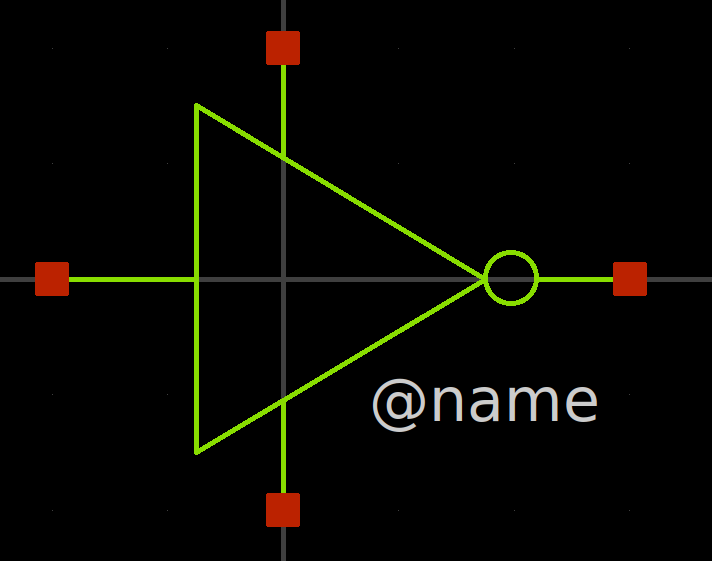
\includegraphics[width=\linewidth]{inverter_sym.png}
            \caption{Inverter symbol created in Xschem.}
        \end{subfigure}
        \begin{subfigure}{0.5\linewidth}
            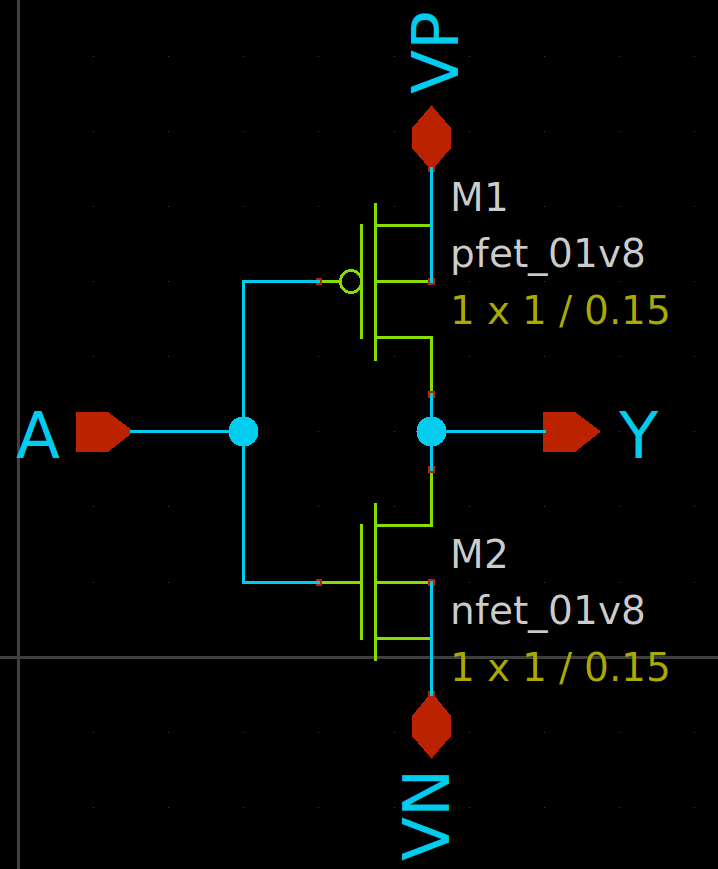
\includegraphics[width=\linewidth]{inverter_sch.png}
            \caption{Inverter schematic created in Xschem.}
        \end{subfigure}
        \caption{Inverter design in Xschem.}
        \label{fig:inv}
    \end{figure}
    To begin with, I implemented an inverter design shown in Figure \ref{fig:inv} as introduced by Professor Minch in his tutorial video.
    \begin{figure}[!ht]
        \begin{subfigure}{0.5\linewidth}
            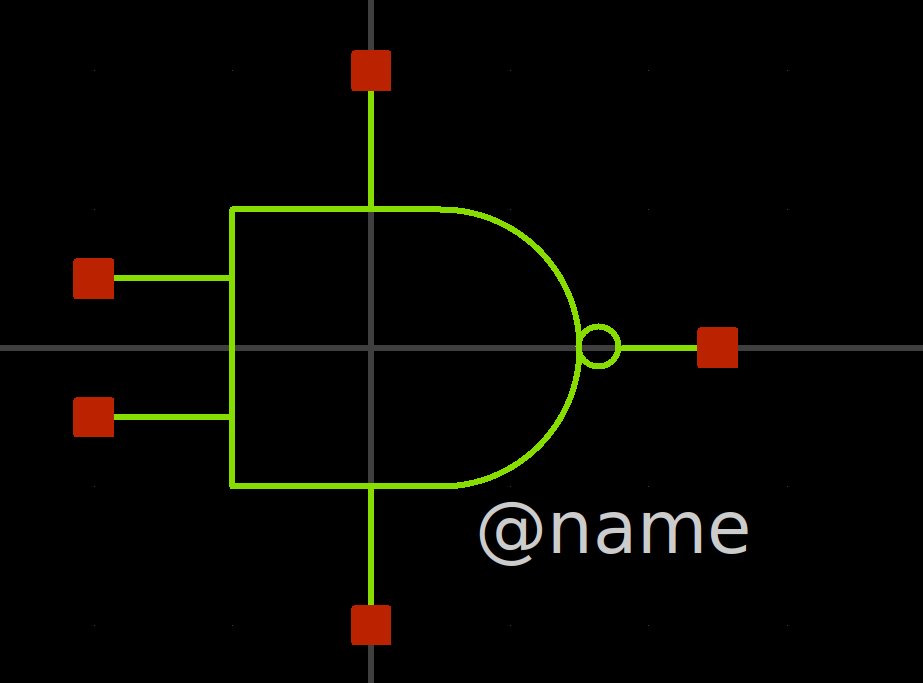
\includegraphics[width=\linewidth]{NAND2_sym.png}
            \caption{NAND2 symbol created in Xschem.}
        \end{subfigure}
        \begin{subfigure}{0.5\linewidth}
            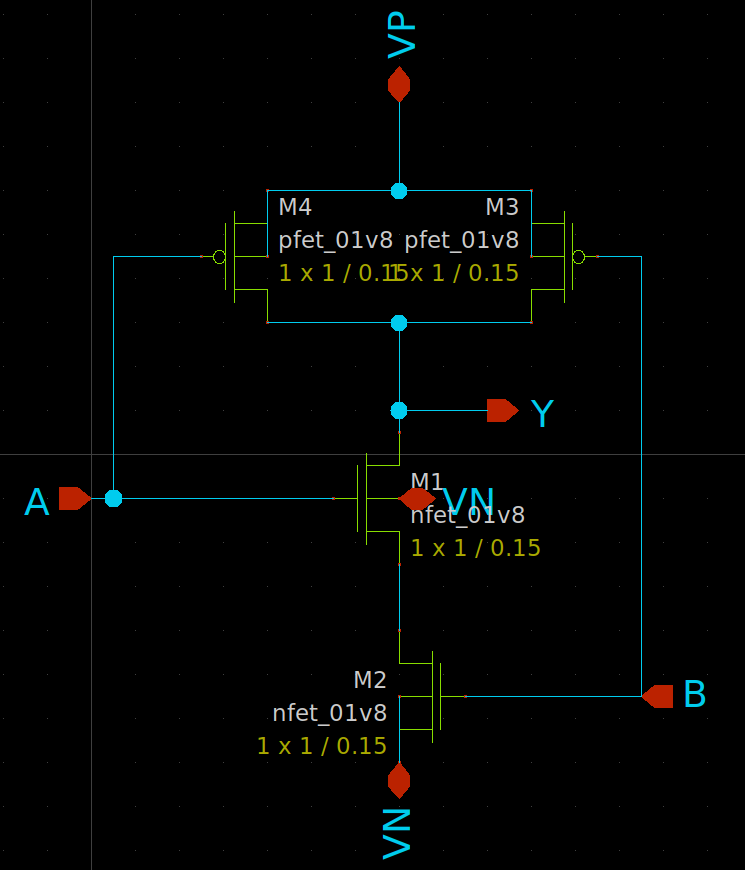
\includegraphics[width=\linewidth]{NAND2_sch.png}
            \caption{NAND2 schematic created in Xschem.}
        \end{subfigure}
        \caption{NAND2 design in Xschem.}
        \label{fig:nand2}
    \end{figure}
    Similarly, I independently created a hierarchy schematic for NAND2 as shown in Figure \ref{fig:nand2}.

    \FloatBarrier
    I created an AND2 gate by inverting the output of NAND2 with the inverter. You can see the test harness of the AND2 gate in Figure \ref{fig:and2}. $V_{DD}$ is set to be 1.8 $V$, and the square waves at NAND2 inputs switches between 0 $V$ and 1.8 $V$. To capture all four possible inputs, $\{00,\ 01,\ 10,\ 11\}$, to be presented to this two-input gate, the square wave at the input node $V_B$ is set to have twice the period of $V_A$. The output node $V_{out}$ is loaded with a 200 $fF$ capacitor as specified.
    \begin{figure}[!ht]
        % \begin{subfigure}{0.5/textwidth}
        %     \
        % \end{subfigure}
        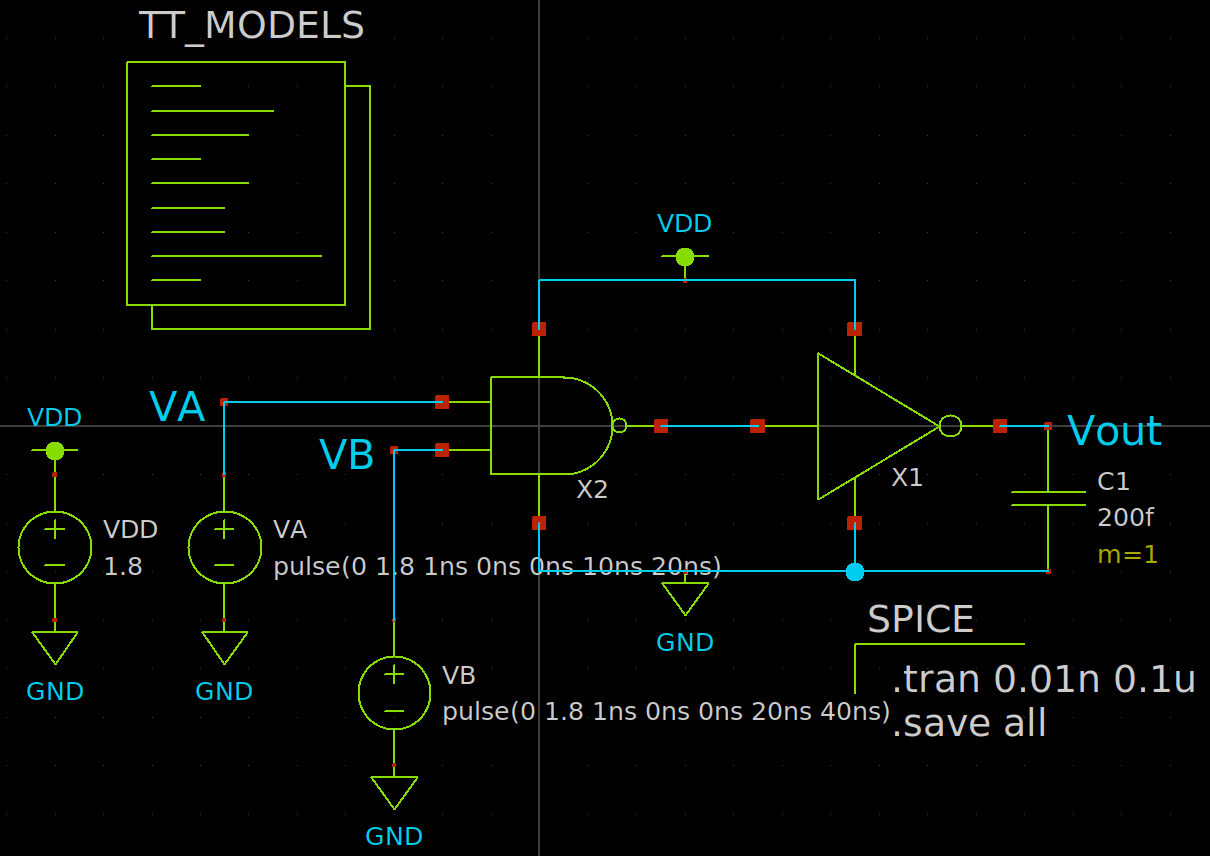
\includegraphics[width=\linewidth]{AND2_harness.png}
        \caption{The simulation setup of a AND2 gate made of a NAND2 and an inverter.}
        \label{fig:and2}
    \end{figure}

    As you can see for the simulation results in Figure \ref{fig:and2res}, the only time where $V_{out}$ outputs high is when both $V_A$ and $V_B$ outputs high. This follows out expectation of how an AND2 gate should behave.
	\begin{figure}[!ht]
        % \begin{subfigure}{0.5/textwidth}
        %     \
        % \end{subfigure}
        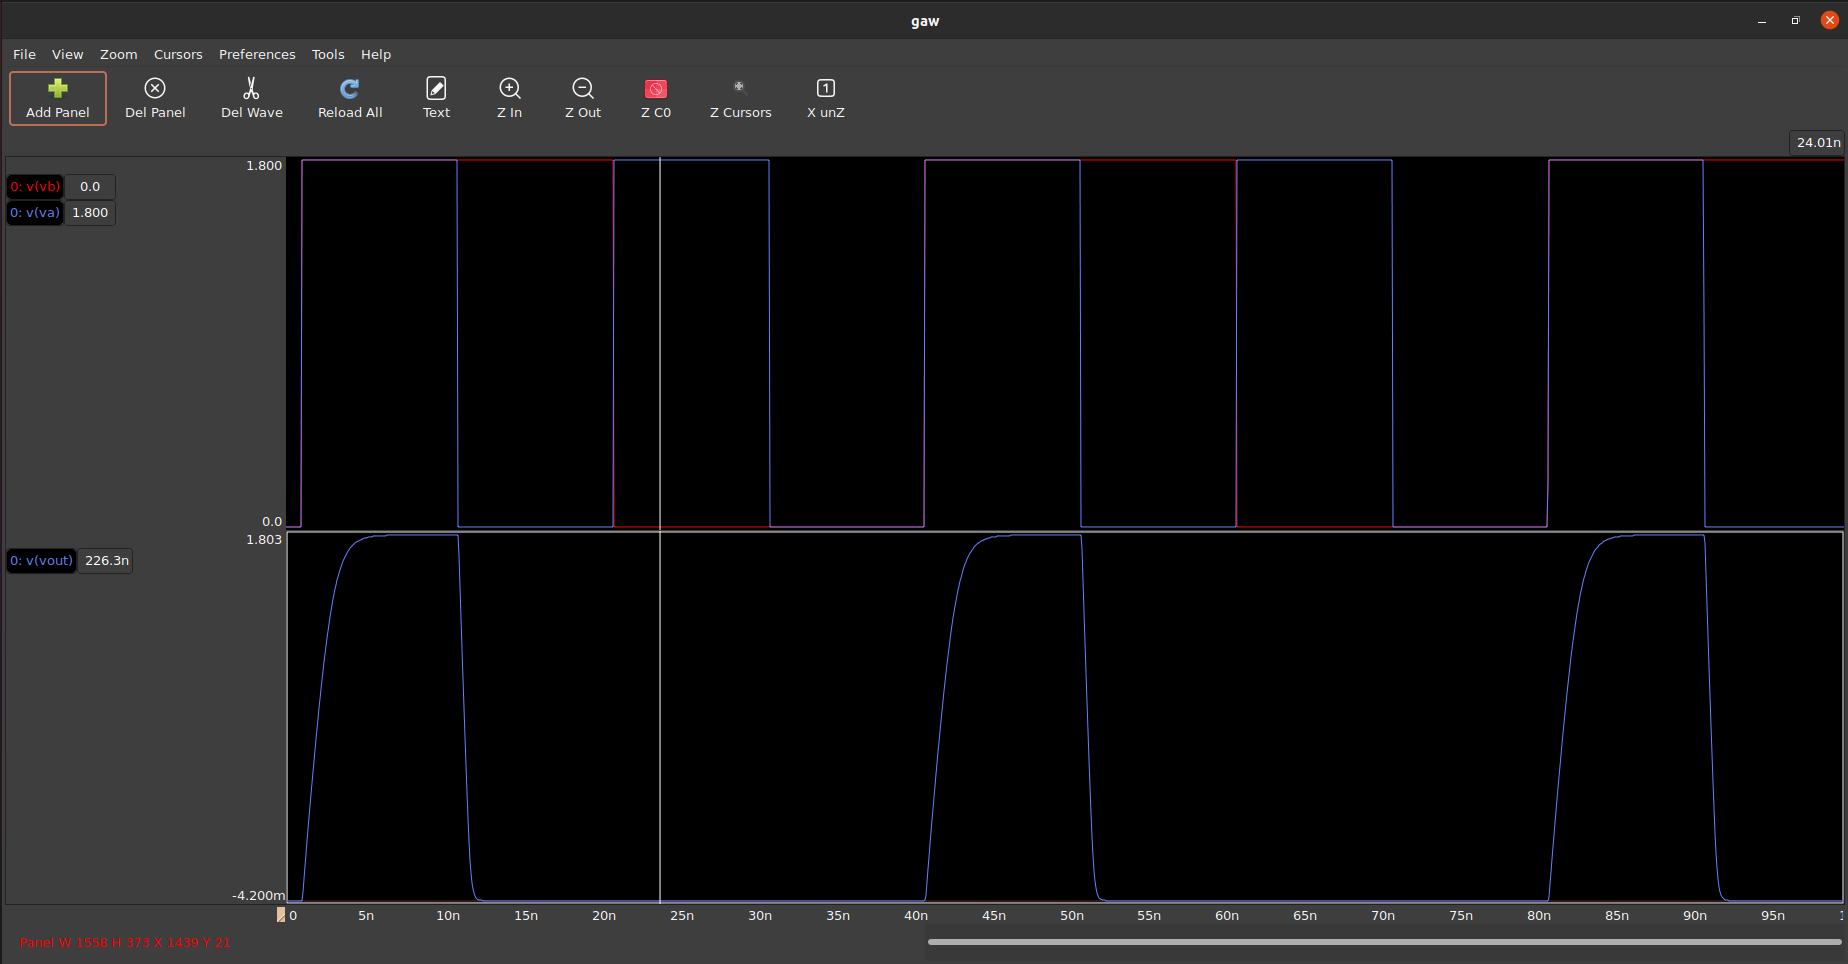
\includegraphics[width=\linewidth]{AND2_sim.png}
        \caption{The simulation AND2 gate behavior view in \textit{gaw}.}
        \label{fig:and2res}
    \end{figure}


\FloatBarrier
\section{Layout Design}
    \begin{figure}[!ht]
        \centering
        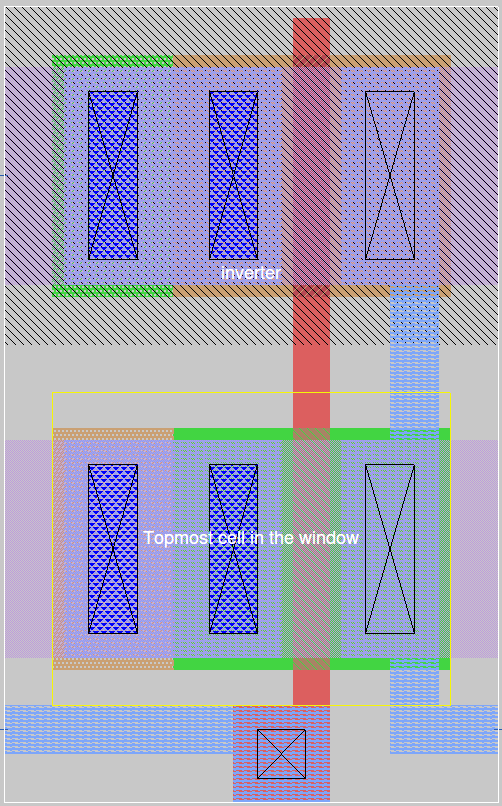
\includegraphics[width=0.8\linewidth]{inverter_mag.png}
        \caption{\textit{Magic} layout of the inverter.}
        \label{fig:invmag}
    \end{figure}
    \begin{figure}[!ht]
        \centering
        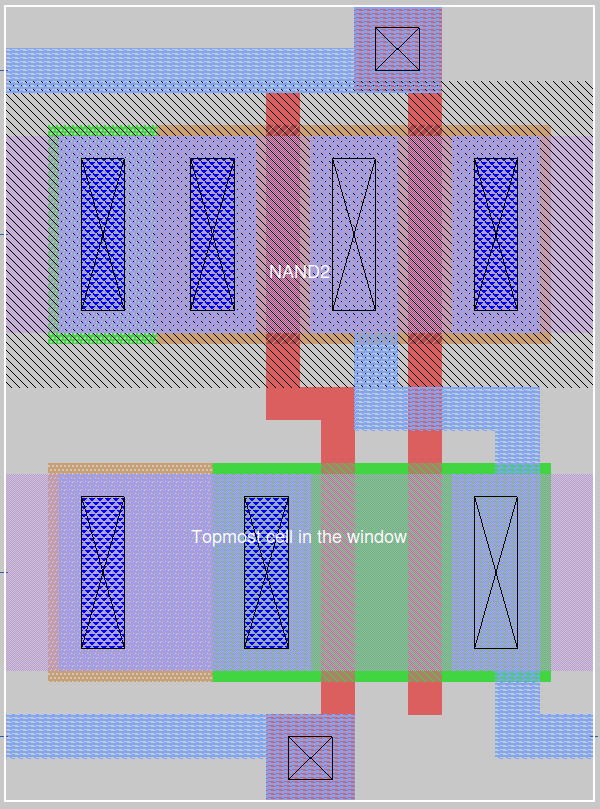
\includegraphics[width=0.8\linewidth]{nand2_mag.png}
        \caption{\textit{Magic} layout of the NAND2.}
        \label{fig:nand2mag}
    \end{figure}
    \begin{figure}[!ht]
        \centering
        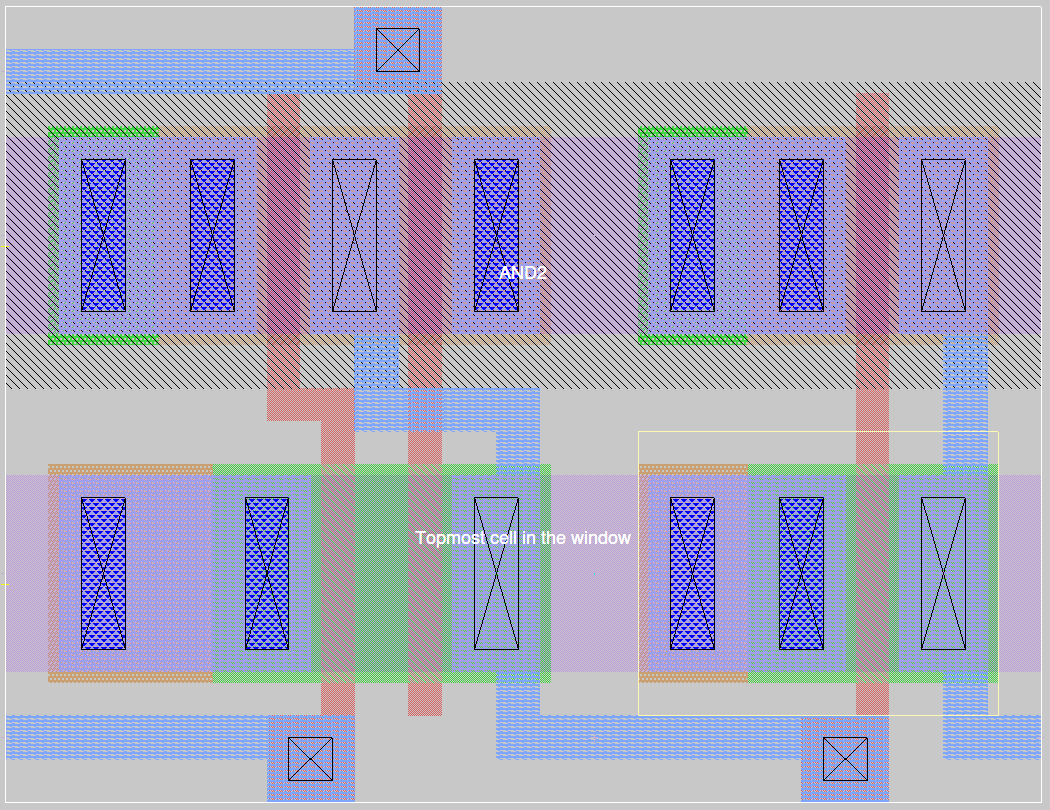
\includegraphics[width=\linewidth]{and2mag.png}
        \caption{\textit{Magic} layout of the AND2 by combining NAND2 and inverter layouts.}
        \label{fig:nand2mag}
    \end{figure}

    \FloatBarrier
    \section{Layout versus Schematic}
    
\end{document}
